\chapter{Recunoașterea obiectelor}


%Recunoașterea obiectelor este o aplicate fundamentala a procesării de imagini și viziunea artificiala.
%De câteva decenii a fost, și încă este un domeniu de cercetare extensiva.
%Termenul "recunoașterea obiectelor" este folosit pentru a descrie multe aplicații și algoritmi.
%Sensul comun, de cele mai multe ori, este: date find cunoștințe despre înfățișarea unor obiecte, una sau mai multe imagini sunt analizate pentru a se stabili dacă exista obiectele în imagine și locația lor.
%Cu toate acestea, fiecare aplicație are cerințe și constrângeri specifice.
%Acest fapt a condus la o mare diversitate de algoritmi.
%De aceea este important ca sa avem la îndemâna biblioteci software, care sa faciliteze dezvoltarea rapida a algoritmilor de recunoaștere a obiectelor.

%Un caz special de recunoaștere a obiectelor apare foarte des, baza de date a modelelor ce trebuiesc recunoscute conține o singura clasa de obiecte, în acest caz sarcina de a detecta prezenta obiectului în imagine este simplificata.

Problema recunoașterii de obiecte se poate exprima în felul următor:
Având o bază de date cu unul sau mai multe modele de obiecte, sa se determine dacă exista obiectul în imagine și, în cazul în care există, să se localizeze.

Unele dintre cele mai relevante lucrări din domeniu sunt: 
\begin{itemize}
	\item "Robust Real-time Object Detection" \cite{Viola01robustreal-time}
	\item "Histograms of Oriented Gradients for Human Detection" \cite{Dalal05histogramsof}
	\item "Object Detection with Discriminatively Trained Part Based Models" \cite{Felzenszwalb_objectdetection}
\end{itemize}

Dacă studiem mai atent algoritmii descriși în aceste lucrări, se observă ca toate au o structură comună și urmăresc o succesiune de operațiuni similare.
Aceste operațiuni sunt următoarele: parcurgerea imaginii în mod spațial la diferite scalări, extragerea de trăsături, clasificarea și post-procesarea rezultatelor.

În continuare se va discuta mai detaliat despre fiecare componentă, iar la sfârșit despre algoritmul de recunoaștere.

\pagebreak
\section{Parcurgerea imaginii în scară și spațiu}

%Obiectele trebuie recunoscute la orice poziție și scara într-o imagine.
Obiectele care trebuie recunoscute pot prezenta deviații de la modelul din baza de date.
Aceste deviații pot fi de natura geometrică: translație, rotație, scalare și perspectivă.

O soluție pentru această problemă ar fi: să se construiască un model care să prezinte toate instanțierile obiectului.
O dificultate a acestei abordări ar fi că nu se pot ști dinainte toate transformările obiectului.
Chiar dacă s-ar ști, se poate deduce că un astfel de model ar putea fi mult prea mare ca să poată fi aplicat practic.

O altă abordare ar fi sa se folosească o reprezentare a imaginii, invariantă la aceste transformări.
Din literatură se știe că o imagine reprezentată în spațiul Fourier este invariantă la translație și o imagine reprezentată în spațiul Log-Polar este invariantă la scalare și rotație\cite{treiber2010introduction}.
Există chiar și o combinație intre aceste două reprezentări numită Fourier-Mellin care este invariantă la toate cele trei transformări.
Totuși s-a observat că utilizarea acestei reprezentări are aplicații limitate, ea fiind folosită mai mult la alinierea imaginilor\cite{treiber2010introduction}.

O altă soluție, poate un pic mai naivă, dar în același timp foarte puternica, este folosirea unei combinații intre o piramidă de imagini și un algoritm de tip fereastră glisantă\footnote{Eng. sliding window}, acestea fiind aplicate pe imagine, nu pe modelul din baza de date.

Folosirea piramidei de imagini și fereastra glisantă ne permit ca în restul algoritmului de recunoaștere să tratăm problema că și cum nu ar exista translații sau scalări, astfel simplificând mult algoritmii aplicați.

O piramidă de imagini este o reprezentare multi-scară.
Piramida de imagini se formează pornind de la o imagine sursă, prin scalari succesive.
Aceste scalari se fac cu un factor ${\alpha > 1, \alpha \in \mathbb{R}}$ și se opresc atunci când se ajunge la o dimensiune minima.
Dimensiunea imaginii la un anumit nivel din piramidă se calculează astfel:
$${
f(D,L) = D \cdot \frac{1}{\alpha^L}
}$$

Unde ${D \in \mathbb{N}^2}$ este dimensiunea imaginii sursă și ${L \in \mathbb{N}^+}$ este nivelul piramidei pentru care dorim sa aflăm dimensiunea.

Se poate vizualiza piramida de imagini în figurile următoare:

\begin{figure}[H]
	\centering
		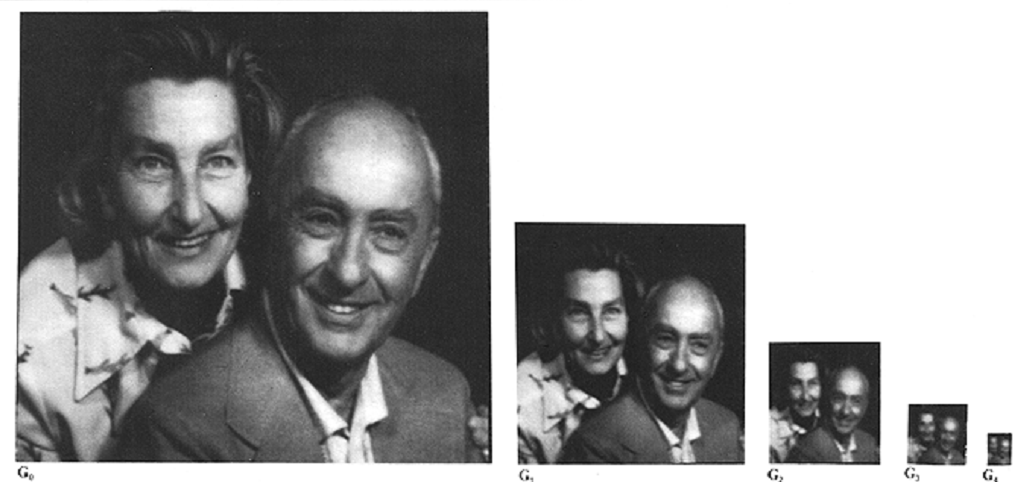
\includegraphics[width=1.0\textwidth]{imagini/pyramid0.png}
		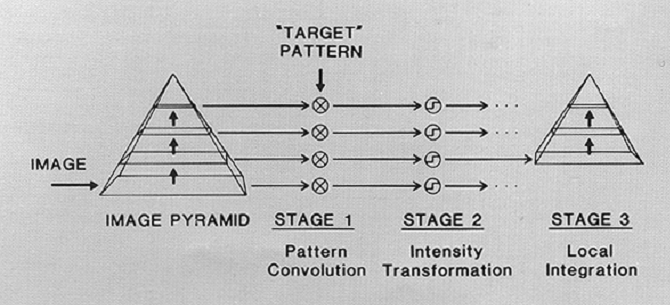
\includegraphics[width=1.0\textwidth]{imagini/pyramid1.png}
	\caption{Piramida de imagini\protect\footnotemark}
	\label{fig:Pyramids_Tutorial_Pyramid_Theory}
\end{figure}

\footnotetext{Pyramid methods in image processing\cite{adelson1984pyramid}.}


Prezentarea formarii piramidei de imagini în pseudo-cod:
\begin{mdframed}
\begin{verbatim}
sursa = citeste_imagine()
alpha = 6/5
dim_min = (100,100)
piramida = [sursa, ]
L=1
cicleaza
  D = sursa.D * 1/(alpha^L)
  daca D < dim_min
    atunci paraseste ciclul
  sfarsit daca
  nivel = scaleaza(sursa, D)
  piramida = insereaza(piramida, nivel)
  L = L + 1
sfarsit cicleaza
\end{verbatim}
\end{mdframed}

Se poate observa că, totuși, acest model nu poate reprezenta toate scările posibile, fiind un model discret.
Această problema poate fi ameliorată prin alegerea unui ${\alpha}$ potrivit și permițând modelului din baza de date să prezinte și el mici variații de scară.

O altă observație ar fi: cu cât ${\alpha}$ este mai mic, cu atât șansele să nimerim scara corectă cresc, dar în același timp creste și consumul de memorie și durata de execuție a algoritmului.
Consumul de memorie poate fi evitat dacă algoritmul se execută într-un mod recursiv, eliminând astfel menținerea explicita a unei liste de imagini în memorie.

Algoritmul fereastră glisantă se folosește pentru a obține invariantă la translație a modelului.
Aici fereastra se refera la o secțiune rectangulară a imaginii.
Fereastra va avea aceeași dimensiune ca și modelul din baza de date.
Fereastra glisantă are ca parametri ${\Delta_x, \Delta_y \geq 1}$, însemnând pasul pe axa ${x}$, respectiv pasul pe axa ${y}$.

Pseudo-cod ferestrei glisante este:
\begin{mdframed}
\begin{verbatim}
dx = 8
dy = 8
I = citeste_imagine()
M = citeste_model()
pentru x de la 0 la dimx(I) - dimx(I)
  pentru y de la 0 la dimy(I) - dimy(M)
    fereastra = sectiune(I, x, y, dimx(M), dimy(M))
    proceseaza(fereastra)
  sfarsit pentru
sfarsit pentru
\end{verbatim}
\end{mdframed}

Se poate vizualiza algoritmul fereastră glisantă în figura următoare:
\begin{figure}[H]
	\centering
		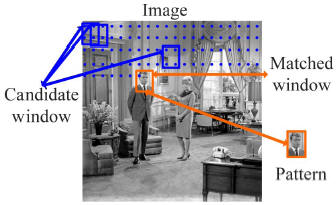
\includegraphics[width=1.00\textwidth]{imagini/sliding_window.png}
	\caption{Parcurgerea fereastră glisantă\protect\footnotemark}
	\label{fig:sliding_window}
\end{figure}
\footnotetext{Imagine din: Segmented Gray-Code Kernels for Fast Pattern Matching\cite{Ouyang2013SegGCK}}


Se observă că aici, ca și în cazul piramidei de imagini, cu cât $x$ și $y$ sunt mai mici, cu atât creste și numărul de ferestre evaluate, ceea ce duce la un timp de execuție mai ridicat.

Complexitatea algoritmului piramidă combinat cu fereastra glisantă este 
$${O((dim_x-\Delta_x) \cdot (dim_y-\Delta_y) \cdot n_{piramida})}$$

\pagebreak
\section{Extragerea de trăsături}

Extragerea de trăsături, în cazul nostru, reprezintă operațiunea de calculare a unei reprezentări a imaginii potrivită pentru recunoaștere.

O imagine este reprezentată ca o matrice de intensități.
Această reprezentare este foarte sensibila la condițiile de iluminare, conține informații irelevante și redundante.
Se poate observa efectul iluminării în figura \ref{fig:efectul_iluminarii}.

\begin{figure}[H]
	\centering
		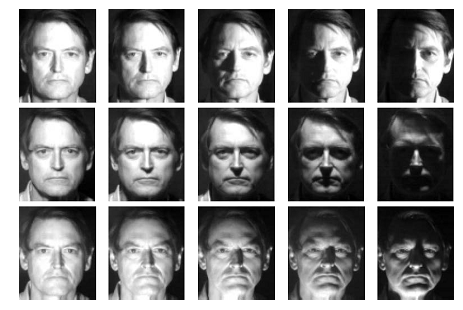
\includegraphics[width=0.90\textwidth]{imagini/efectul_iluminarii.png}
	\caption{Efectul iluminării\protect\footnotemark}
	\label{fig:efectul_iluminarii}
\end{figure}
\footnotetext{Sursă imagine: Computer vision: algorithms and applications\cite{szeliski2010computer}}


Există modalități de a remedia efectul iluminării, cum ar fi egalizarea histogramei(fig. \ref{fig:egalizarea_histogrameis}).
O altă modalitate ar fi să se folosească o reprezentare pe bază de gradienți care sunt invarianți la iluminare.

\begin{figure}[H]
	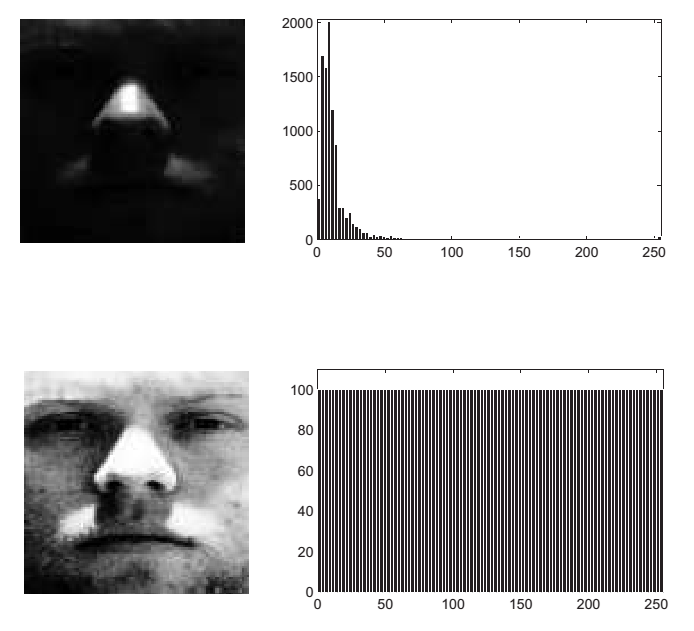
\includegraphics[width=1.0\textwidth]{imagini/histogram_equalization.png}
	\caption{Egalizarea Histogramei\protect\footnotemark}
	\label{fig:egalizarea_histogrameis}
\end{figure}
\footnotetext{Sursă imagine: Histogram remapping as a preprocessing step for robust face recognition\cite{vstruc2009histogram}}


Efectul informațiilor irelevante și redundante poate fi ameliorat folosind tehnici de reducere a dimensionalității, cum ar fi analiza componentelor principale\footnote{Eng. PCA, principal component analisys}(fig. \ref{fig:fig_pca_principal_component_analysis}) sau transformata cosinus discretă(fig. \ref{fig:take_DCT}).

\begin{figure}[H]
	\centering
		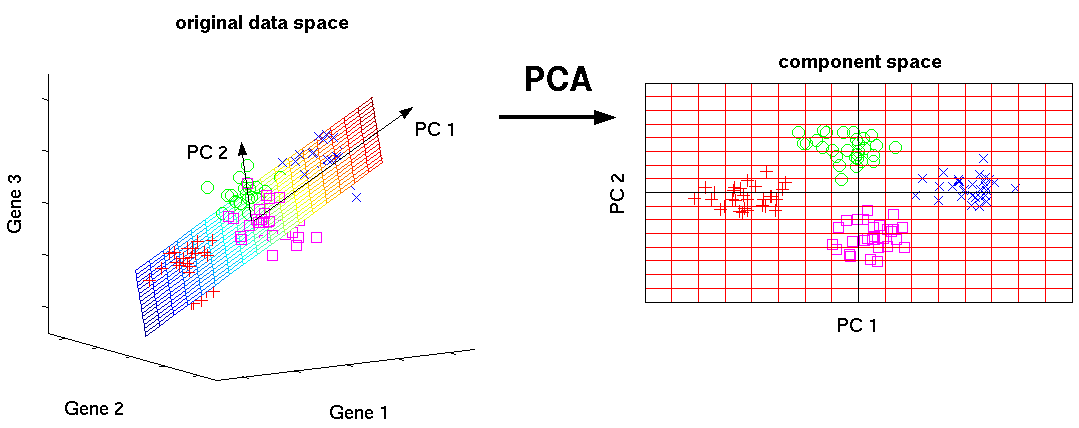
\includegraphics[width=0.90\textwidth]{imagini/fig_pca_principal_component_analysis.png}
	\caption{Analiza componentelor principale\protect\footnotemark}
	\label{fig:fig_pca_principal_component_analysis}
\end{figure}
\footnotetext{Sursă imagine: \url{http://phdthesis-bioinformatics-maxplanckinstitute-molecularplantphys.matthias-scholz.de}}

\begin{figure}[H]
	\centering
		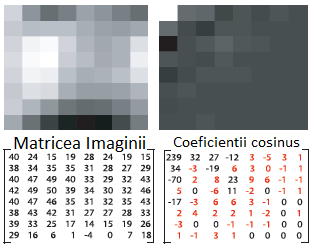
\includegraphics[width=0.90\textwidth]{imagini/take_DCT.png}
	\caption{Transformata cosinus\protect\footnotemark}
	\label{fig:take_DCT}
\end{figure}
\footnotetext{Sursă imagine: \url{http://cnx.org/content/m13173/1.6/}}


Totuși, nici una dintre reprezentările menționate mai sus nu tratează problema discriminării, adică: dacă două imagini conțin același obiect atunci și reprezentările lor trebuie sa fie apropiate, iar dacă sunt imagini ale unor obiecte diferite atunci reprezentările lor trebuie sa fie distanțate.

Aici intervine ceea ce se numește ingineria trăsăturilor\footnote{Eng. Feature Engineering} care, folosind cunoștințe din fizică, biologie sau chiar neurologie , construiește reprezentări mult mai favorabile recunoașterii.
Câteva dinte cele mai cunoscute trăsături sunt HAAR\cite{Viola01robustreal-time}, SIFT\cite{Lowe99objectrecognition} și HOG\cite{Dalal05histogramsof}.

Valoarea unei trăsături HAAR este diferența dintre suma pixelilor din dreptunghiul negru și suma pixelilor din dreptunghiul alb, normalizată la aria celor două.
\begin{figure}[H]
	\centering
		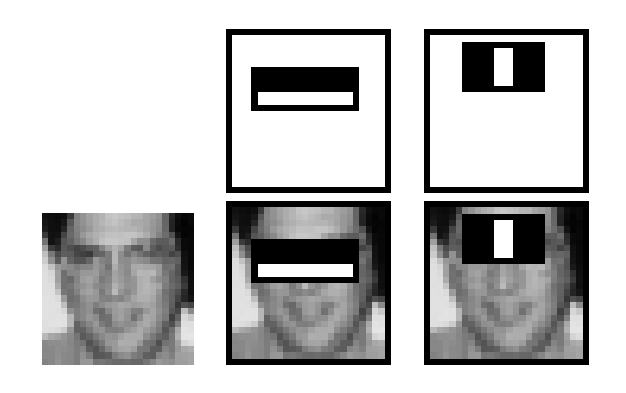
\includegraphics[width=0.50\textwidth]{imagini/haar0.png}
		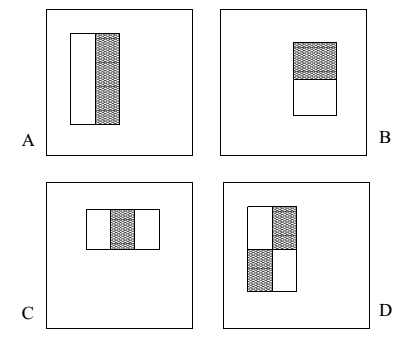
\includegraphics[width=0.48\textwidth]{imagini/haar1.png}
	\caption{Trasaturi HAAR\protect\footnotemark}
	\label{fig:haarfeatures}
\end{figure}
\footnotetext{Sursă imagine: Robust Real-time Object Detection\cite{Viola01robustreal-time}}

HOG, sau histograma orientărilor de gradienți, se calculează divizând imaginea în zone mai mici, numite celule, apoi se calculează histograma de orientări a gradienților din aceste zone. 
Concatenarea acestor histograme reprezintă trăsătura HOG.
\begin{figure}[H]
	\centering
		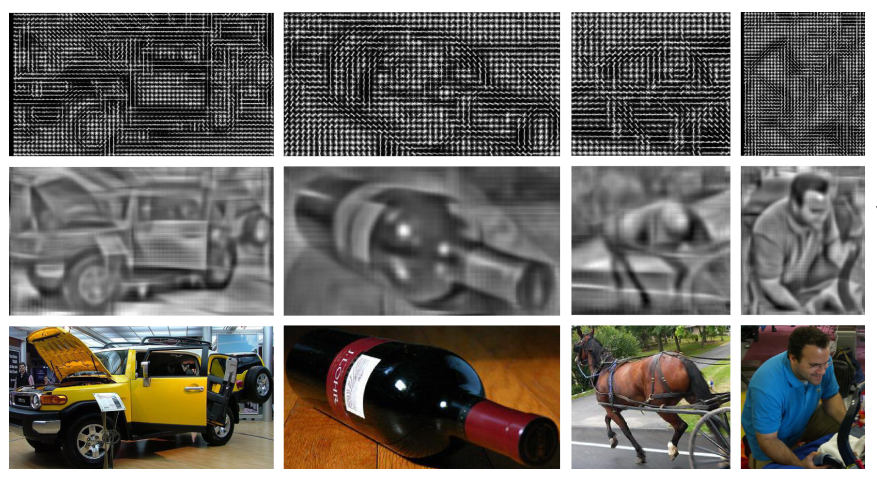
\includegraphics[width=0.80\textwidth]{imagini/hog0.png}
	\caption{Trasaturi HOG\protect\footnotemark}
	\label{fig:hog0}
\end{figure}
\footnotetext{Sursă imagine: HOGgles: Visualizing Object Detection Features\cite{vondrick2013hoggles}}

Descriptorul SIFT este similar cu HOG, acesta fiind în plus și invariant la rotație.
\begin{figure}[H]
	\centering
		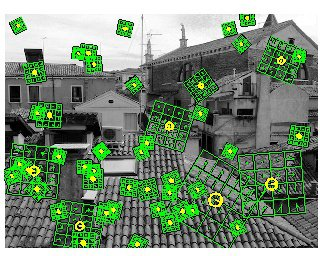
\includegraphics[width=0.80\textwidth]{imagini/sift0.jpg}
	\caption{Descriptorul SIFT\protect\footnotemark}
	\label{fig:sift}
\end{figure}
\footnotetext{Sursa imagine: \url{http://www.vlfeat.org/overview/sift.html}}

Recent a apărut o nouă abordare în ceea ce privește extragerea de trăsături.
Aceasta folosește reprezentarea crudă a imaginii, adică matricea de intensități a pixelilor și se bazează pe algoritmul de clasificare să extragă trăsături mai puternice, un exemplu fiind rețeaua neuronală convolutională\cite{lecun-98}.

\section{Clasificare}

Din perspectiva recunoașterii obiectelor, clasificarea se va realiza cu ajutorul unei funcții care evaluează un vector de trăsături și decide dacă este sau nu obiectul pe care încercam sa îl recunoaștem. 
Acest tip de clasificare se numește clasificare binară, fiindcă răspunsul nu poate lua decât două valori.

Această funcție de decizie poate fi, în cazurile cele mai simple, o funcție de prag peste o distantă euclidiană sau chiar o rețea neuronală cu sute de neuroni.

În cazul nostru această funcție este rezultatul unui algoritm de învățare automată\footnote{Eng. Machine Learning}.
Învățarea automată, o ramura a inteligentei artificiale, este preocupată cu studiul și construcția sistemelor care pot învață din date.
Algoritmii de învățare automată sunt împărțiți în multe categorii, însa noi ne vom axa doar pe cei de învățare supervizată.
Se numesc algoritmi de învățare supervizată acei algoritmi care folosesc la antrenament seturi de perechi de date ${(x,y)}$ unde ${x}$ reprezintă trăsăturile sau atributele unui exemplar, iar ${y}$ reprezintă răspunsul dorit. 
După ce a avut loc învățarea, algoritmul va fi capabil să producă un răspuns și în cazul unor exemplare pe care nu le-a mai întâlnit, de aceea în literatura de specialitate clasificatorii se mai numesc și predictori.

Scopul învățării automate, dacă privim problema din punct de vedere geometric, este acela de a găsi un plan care să separe cele două clase intre ele(fig: \ref{fig:fig_clasificare}).

\begin{figure}[h]
	\centering
		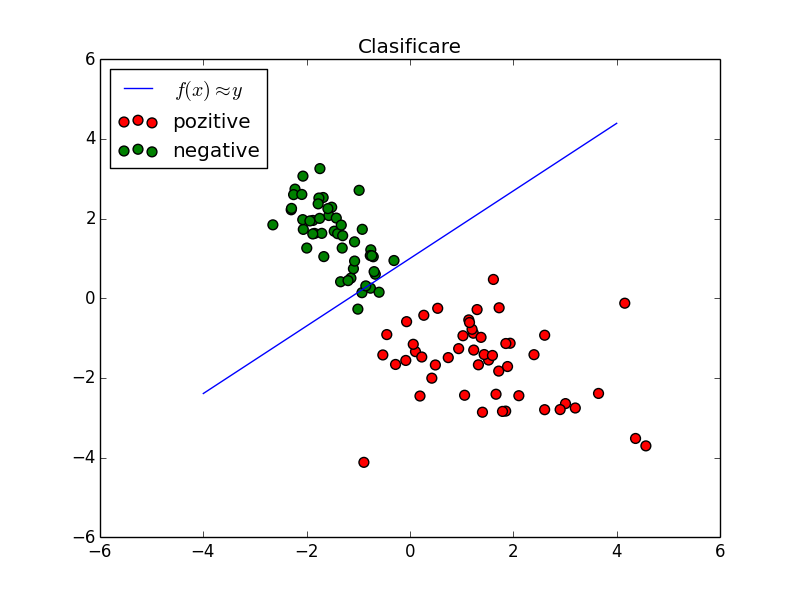
\includegraphics[width=0.8\textwidth]{imagini/fig_clasificare2.png}
	\caption{Clasificare}
	\label{fig:fig_clasificare}
\end{figure}

Cel mai des întâlniți algoritmi de învățare în viziunea artificială sunt: automatul cu vectori de suport\footnote{Eng. Support Vector Machines}\cite{suykens1999least} și rețeaua neuronală.

\pagebreak
\section{Post-procesarea rezultatelor}

O situație foarte des întâlnită în cazul algoritmilor de recunoaștere a imaginilor este că același obiect este detectat de mai multe ori.
Aceste detecții sunt suprapuse și se datorează faptului ca modelul învățat recunoaște și obiecte cu mici translații și scalări.
Totuși, se dorește ca fiecare obiect prezent în imagine sa fie detectat doar o singură dată.
Acest lucru se realizează cu ajutorul unui algoritm de grupare a detecțiilor suprapuse.
\begin{figure}[h]
	\centering
		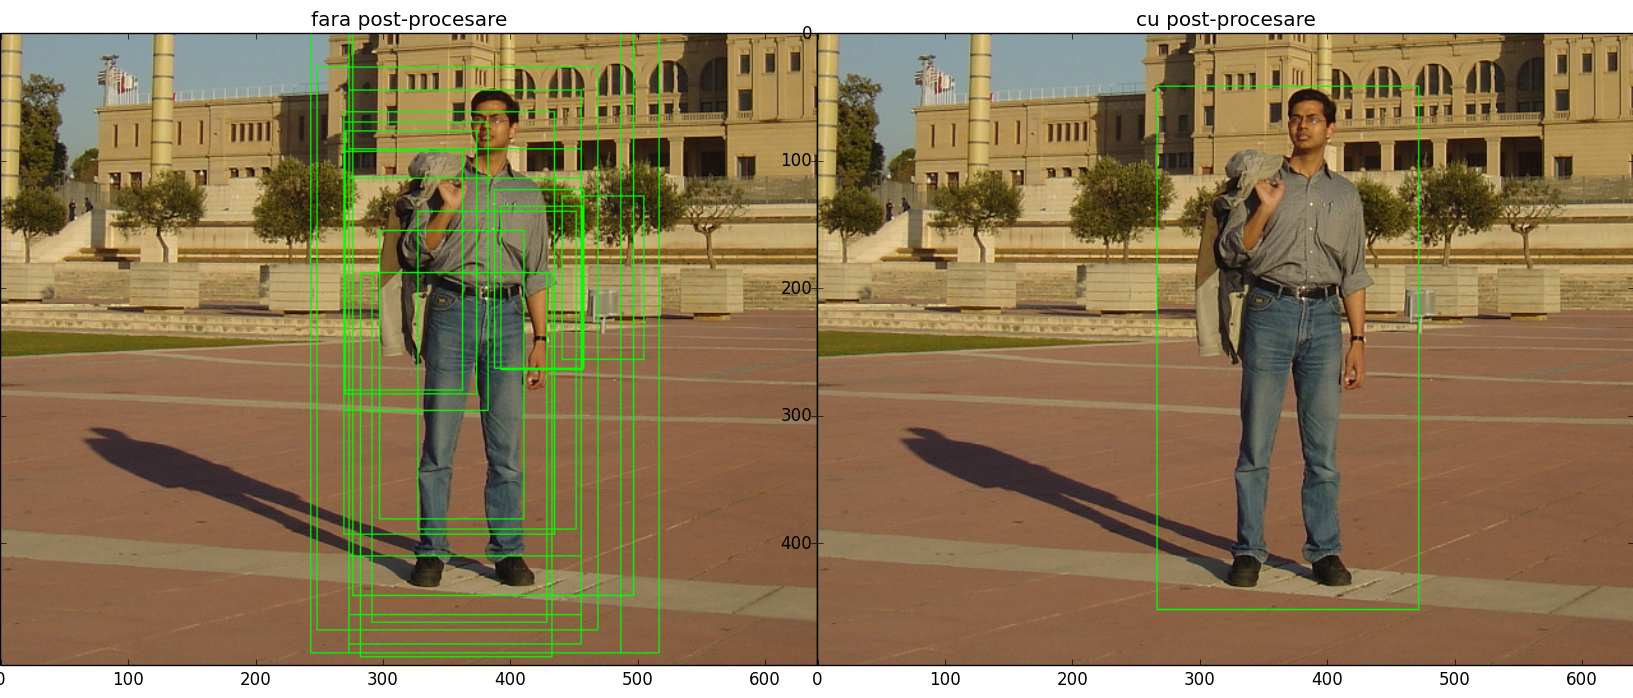
\includegraphics[width=0.8\textwidth]{imagini/nms.png}
	\caption{Efectul post-procesării}
	\label{fig:nms}
\end{figure}


\pagebreak
\section{Algoritmul de recunoaștere}

Algoritmul de recunoaștere a obiectelor poate fi implementat folosind componentele descrise pe parcursul acestui capitol, urmărind pseudo-codul:
\begin{mdframed}
\begin{verbatim}

detectii = lista()

I = citeste_imaginea()
P = construieste_piramida(I)

pentru fiecare nivel din P
  pentru fiecare fereastra din extrage_ferestele(P)
    trasaturi = extrage_trasaturi(fereastra)
    raspuns = clasificare(trasaturi)
    daca rasuns este afirmativ atunci
      detectii = adauga(detectii, locatie(fereastra))
    sfarsit daca
  sfarsit
sfarsit

detectii = grupare_suprapuse(detectii)

\end{verbatim}
\end{mdframed}

\section{Antrenarea algoritmului de recunoaștere}

Pentru antrenarea unui algoritm de recunoaștere a obiectelor avem nevoie de o bază de date cu două seturi de imagini.
Un set va conține imagini decupate cu obiectul pe care dorim sa îl recunoaștem, iar al doilea va fi constituit din imagini care nu conțin obiectul.
Aceste seturi se numesc setul de exemplare pozitive, respectiv negative.
Setul de pozitive este adus la o mărime comună prin redimensionare, iar setul de negative este folosit în întregime.

Pentru că setul de negative poate conține chiar și milioane de exemplare, nu este practic ca la antrenare sa se folosească toate exemplarele posibile.
Se va încerca extragerea doar a acelor exemplare care contribuie la îmbunătățirea antrenamentului.
Printr-un proces iterativ de antrenări succesive, numit "bootstrapping", din setul de imagini negative se vor extrage exemplare folosind scanarea în scara și spațiu de la algoritmul de recunoaștere.
În prima iterație se extrage un număr de exemple negative specificat de către utilizator și se antrenează clasificatorul.
Apoi, folosind clasificatorul antrenat la pasul anterior, se scanează imaginile negative.
Fiecare exemplar negativ care a fost clasificat ca fiind pozitiv este adăugat în lista de antrenare și se antrenează clasificatorul din nou.
Pasul acesta se repetă de un număr de ori specificat de utilizator, sau pană când nu se mai pot extrage exemplare negative din setul de date.
Acest algoritm va atinge performantele unui algoritm naiv, antrenat cu toate exemplarele, folosind un număr mult mai mic de exemplare și într-un timp mult mai scurt.

\begin{mdframed}
\begin{verbatim}

P = citeste_setul_de_exemplare_positive()
N = citeste_setul_de_exemplare_negative()

X = lista()
y = lista()

X = adauga(X, P)
y = adauga(y, selecteaza_aleator(N))

Cls = antreneaza_clasificator(X,y)

iter = citeste_nr_iteratii()

pentru i = 1 pana la iter
  pentru I din N
    P = construieste_piramida(I)
    pentru fiecare nivel din P
      pentru fiecare fereastra din extrage_ferestele(P)
        xi = extrage_trasaturi(xi)
        raspuns = clasificare(Cls, xi)
        daca rasuns este 'afirmativ' atunci
          X = adauga(X, xi)
          y = adauga(y, 'negativ')
        sfarsit daca
      sfarsit
    sfarsit
  sfarsit
  
  Cls = antreneaza_clasificator(X,y)
sfarsit
\end{verbatim}
\end{mdframed}



















